%package list
\documentclass{article}
\usepackage[top=3cm, bottom=3cm, outer=3cm, inner=3cm]{geometry}
\usepackage{multicol}
\usepackage{graphicx}
\usepackage{url}
%\usepackage{cite}
\usepackage{hyperref}
\usepackage{array}
%\usepackage{multicol}
\newcolumntype{x}[1]{>{\centering\arraybackslash\hspace{0pt}}p{#1}}
\usepackage{natbib}
\usepackage{pdfpages}
\usepackage{multirow}    
\usepackage[normalem]{ulem}
\useunder{\uline}{\ul}{}
\usepackage{svg}
\usepackage{xcolor}
\usepackage{listings}
\lstdefinestyle{ascii-tree}{
    literate={├}{|}1 {─}{--}1 {└}{+}1 
  }

\lstset{basicstyle=\ttfamily,
  showstringspaces=false,
  commentstyle=\color{red},
  keywordstyle=\color{blue}
}
%\usepackage{booktabs}
\usepackage{caption}
\usepackage{subcaption}
\usepackage{float}
\usepackage{array}

\usepackage{enumitem}


\newcolumntype{M}[1]{>{\centering\arraybackslash}m{#1}}
\newcolumntype{N}{@{}m{0pt}@{}}


%%%%%%%%%%%%%%%%%%%%%%%%%%%%%%%%%%%%%%%%%%%%%%%%%%%%%%%%%%%%%%%%%%%%%%%%%%%%
%%%%%%%%%%%%%%%%%%%%%%%%%%%%%%%%%%%%%%%%%%%%%%%%%%%%%%%%%%%%%%%%%%%%%%%%%%%%
\newcommand{\itemEmail}{vmaldonadov@unsa.edu.pe}
\newcommand{\itemStudent}{Victor Gonzalo Maldonado Vilca}
\newcommand{\itemCourse}{Programación Web 2}
\newcommand{\itemCourseCode}{1702122}
\newcommand{\itemSemester}{III}
\newcommand{\itemUniversity}{Universidad Nacional de San Agustín de Arequipa}
\newcommand{\itemFaculty}{Facultad de Ingeniería de Producción y Servicios}
\newcommand{\itemDepartment}{Departamento Académico de Ingeniería de Sistemas e Informática}
\newcommand{\itemSchool}{Escuela Profesional de Ingeniería de Sistemas}
\newcommand{\itemAcademic}{2024 - A}
\newcommand{\itemInput}{Del 9 de abril de 2024}
\newcommand{\itemOutput}{Al 15 de junio de 2024}
\newcommand{\itemPracticeNumber}{08}
\newcommand{\itemTheme}{Django}
%%%%%%%%%%%%%%%%%%%%%%%%%%%%%%%%%%%%%%%%%%%%%%%%%%%%%%%%%%%%%%%%%%%%%%%%%%%%
%%%%%%%%%%%%%%%%%%%%%%%%%%%%%%%%%%%%%%%%%%%%%%%%%%%%%%%%%%%%%%%%%%%%%%%%%%%%

\usepackage[english,spanish]{babel}
\usepackage[utf8]{inputenc}
\AtBeginDocument{\selectlanguage{spanish}}
\renewcommand{\figurename}{Figura}
\renewcommand{\refname}{Referencias}
\renewcommand{\tablename}{Tabla} %esto no funciona cuando se usa babel
\AtBeginDocument{%
	\renewcommand\tablename{Tabla}
}

\usepackage{fancyhdr}
\pagestyle{fancy}
\fancyhf{}
\setlength{\headheight}{30pt}
\renewcommand{\headrulewidth}{1pt}
\renewcommand{\footrulewidth}{1pt}
\fancyhead[L]{\raisebox{-0.2\height}{
\includegraphics[width=3cm]{img/logo_episunsa.png}}}
\fancyhead[C]{\fontsize{7}{7}\selectfont	\itemUniversity \\ \itemFaculty \\ \itemDepartment \\ \itemSchool \\ \textbf{\itemCourse}}
\fancyhead[R]{\raisebox{-0.2\height}{
\includegraphics[width=1.2cm]{img/logo_abet}}}
\fancyfoot[L]{Victor M.}
\fancyfoot[C]{\itemCourse}
\fancyfoot[R]{Página \thepage}

% para el codigo fuente
\usepackage{listings}
\usepackage{color, colortbl}
\definecolor{dkgreen}{rgb}{0,0.6,0}
\definecolor{gray}{rgb}{0.5,0.5,0.5}
\definecolor{mauve}{rgb}{0.58,0,0.82}
\definecolor{codebackground}{rgb}{0.95, 0.95, 0.92}
\definecolor{tablebackground}{rgb}{0.8, 0, 0}

\lstset{frame=tb,
	language=bash,
	aboveskip=3mm,
	belowskip=3mm,
	showstringspaces=false,
	columns=flexible,
	basicstyle={\small\ttfamily},
	numbers=none,
	numberstyle=\tiny\color{gray},
	keywordstyle=\color{blue},
	commentstyle=\color{dkgreen},
	stringstyle=\color{mauve},
	breaklines=true,
	breakatwhitespace=true,
	tabsize=3,
	backgroundcolor= \color{codebackground},
}

\begin{document}
	
	\vspace*{10px}
	
	\begin{center}	
		\fontsize{17}{17} \textbf{ Informe de Laboratorio 08}
	\end{center}
	\centerline{\textbf{\Large Tema: \itemTheme}}
	%\vspace*{0.5cm}	

	\begin{flushright}
		\begin{tabular}{|M{2.5cm}|N|}
			\hline 
			\rowcolor{tablebackground}
			\color{white} \textbf{Nota}  \\
			\hline 
			     \\[30pt]
			\hline 			
		\end{tabular}
	\end{flushright}	

	\begin{table}[H]
		\begin{tabular}{|x{4.7cm}|x{4.8cm}|x{4.8cm}|}
			\hline 
			\rowcolor{tablebackground}
			\color{white} \textbf{Estudiante} & \color{white}\textbf{Escuela}  & \color{white}\textbf{Asignatura}   \\
			\hline 
			{\itemStudent \par \itemEmail} & \itemSchool & {\itemCourse \par Semestre: \itemSemester \par Código: \itemCourseCode}     \\
			\hline 			
		\end{tabular}
	\end{table}		
	
	\begin{table}[H]
		\begin{tabular}{|x{4.7cm}|x{4.8cm}|x{4.8cm}|}
			\hline 
			\rowcolor{tablebackground}
			\color{white}\textbf{Tarea} & \color{white}\textbf{Tema}  & \color{white}\textbf{Duración}   \\
			\hline 
			\itemPracticeNumber & \itemTheme & 2 horas   \\
			\hline 
		\end{tabular}
	\end{table}
	
	\begin{table}[H]
		\begin{tabular}{|x{4.7cm}|x{4.8cm}|x{4.8cm}|}
			\hline 
			\rowcolor{tablebackground}
			\color{white}\textbf{Semestre académico} & \color{white}\textbf{Fecha de inicio}  & \color{white}\textbf{Fecha de entrega}   \\
			\hline 
			\itemAcademic & \itemInput &  \itemOutput  \\
			\hline 
		\end{tabular}
	\end{table}
%%%%%%%%%%%%%%%%%%%%

  \section{Introducción}
    Django es un poderoso framework de desarrollo web en Python que simplifica la gestión de bases de datos a 
    través de su sistema ORM. Este sistema incluye la capacidad de manejar relaciones de uno a muchos y muchos 
    a muchos, además de generar PDFs y enviar correos electrónicos. Las relaciones de uno a muchos se implementan 
    utilizando ForeignKey, lo que permite que una fila de una tabla esté vinculada a múltiples filas de otra tabla. 
    Por otro lado, las relaciones de muchos a muchos se manejan con ManyToManyField, lo que permite interacciones 
    complejas entre tablas. Para la generación de PDFs, se pueden usar bibliotecas como WeasyPrint que transforman 
    plantillas HTML en documentos PDF. El envío de correos electrónicos es facilitado por django.core.mail, permitiendo 
    enviar correos electrónicos de manera programada. Estas funcionalidades hacen de Django una herramienta versátil y 
    eficiente para el desarrollo de aplicaciones web completas.

%%%%%%%%%%%%%%%%%%%%

  \section{Objetivos}
    \begin{itemize}
      \item Implementar en una aplicación en Django el manejo de Bases de datos.
      \item Utilizar una tabla y relacionarla con muchas tablas.
      \item Utilizar muchas tablas y relacionarlas con muchas tablas.
      \item Implementar el envío de emails y la impresión de pdfs desde una aplicación Django
    \end{itemize}

%%%%%%%%%%%%%%%%%%%%
 
	\section{Tarea}
    \begin{itemize}
      \item Actividades
        \begin{enumerate}
          \item Crear un proyecto en Django
          \item Siga los pasos de los videos para poder implementar la aplicación de Relación de Uno a muchos en una Base de Datos, muchos a muchos, impresión de pdfs y envío de emails.
          \item Use git y haga los commits necesarios para manejar correctamente la aplicación.
        \end{enumerate}
      \item Ejercicios Propuestos
        \begin{enumerate}
          \item Deberán replicar la actividad de los videos donde se trabaja con Relacion de uno a muchos, de muchos a muchos, impresión de pdfs y envío de emails;  adecuándolo desde un proyecto en blanco Django.
          \item Para ello crear una carpeta dentro del proyecto github colaborativo con el docente, e informar el link donde se encuentra.  
          \item Eres libre de agregar CSS para decorar tu trabajo.
          \item Ya sabes que el trabajo con Git es obligatorio.  Revisa los videos entregados.
        \end{enumerate}
    \end{itemize}
 
%%%%%%%%%%%%%%%%%%%% 
 
  \section{Entregables}
    \begin{itemize}
      \item Informe hecho en Latex
      \item URL: Repositorio GitHub
      \item Link de Vídeo Explicativo (Youtube o flipgrid)
    \end{itemize}
  
%%%%%%%%%%%%%%%%%%%%    
		
	\section{Equipos, materiales y temas utilizados}
    \begin{itemize}
      \item Proyectos de Django
      \item Aplicaciones en Django
      \item Relaciones entre Tablas
      \item Envío de Emails e impresión de PDFs
    \end{itemize}

%%%%%%%%%%%%%%%%%%%%

  \section{URL de Repositorio Github}
  \begin{itemize}
    \item URL del Repositorio GitHub
    \item \url{https://github.com/Victor-Gonzalo-Maldonado-Vilca/Django_Lab08.git}
  \end{itemize}
  
%%%%%%%%%%%%%%%%%%%%

	\section{Link de Video}
  \begin{itemize}
    \item Link del Vídeo Explicativo
    \item \textbf{Youtube: } \url{https://www.youtube.com/watch?v=0j3u3PcELEk}
    \item \textbf{flipgrid: } \url{https://flip.com/s/YSxoPgTJ6DyZ}
  \end{itemize}

%%%%%%%%%%%%%%%%%%%%

  \section{Metodología}
  
%%%%%%%%%%%%

  \subsection{Creación del entorno de Trabajo}
  
%%%%%%

  \subsubsection{Configuración de la carpeta de trabajo}
  \begin{lstlisting}[language=, caption={Creación del Directorio}]
    mkdir lab08 && cd lab08
    virtualenv -p python3 .
    Scripts/activate
    pip install Django
  \end{lstlisting}
  
%%%%%%

  \subsubsection{Creación carpeta del proyecto}
  \begin{lstlisting}[language=, caption={Carpeta src}]
    mkdir src && cd src
  \end{lstlisting}
  
%%%%%%

  \subsubsection{Inicializar git}
  \begin{lstlisting}[language=, caption={Inicializar git}]
    git init
  \end{lstlisting}
  
%%%%%%

  \subsubsection{Crear .gitignore}
  Seguimos el siguiente Repositorio \url{https://github.com/django/django/blob/main/.gitignore}
  
%%%%%%%%%%%%
  
  \subsection{Creacion del proyecto y apps}
  
%%%%%%

  \subsubsection{Crear Proyectos}
  \begin{lstlisting}[language=, caption={Crear proyecto}]
    django-admin startproject model_examples
    django-admin startproject pdf_printing
    django-admin startproject email_project
  \end{lstlisting}
  
%%%%%%

  \subsubsection{Crear App en el Proyecto model examples}
    \begin{lstlisting}[language=, caption={Crear App}]
      python manage.py startapp example
    \end{lstlisting}
  
%%%%%%

  \subsubsection{Crear App en el Proyecto email project}
  \begin{lstlisting}[language=, caption={Crear App}]
    python manage.py startapp email_app
  \end{lstlisting}
  
%%%%%%%%%%%%

  \subsection{Uso de Xampp como base de Datos}
    \textit{Se especificará como se logro en desarrollo de trabajo del video 5 'Database-settings'}
    \begin{figure}[H]
      \centering
      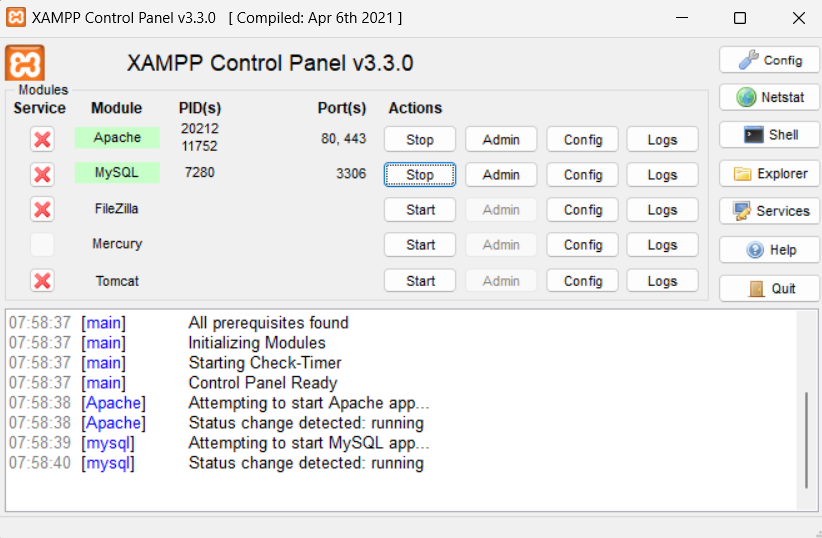
\includegraphics[width=1\textwidth, keepaspectratio]{img/xampp1.png}
      \caption{Xampp Panel Control}
    \end{figure}
    \begin{figure}[H]
      \centering
      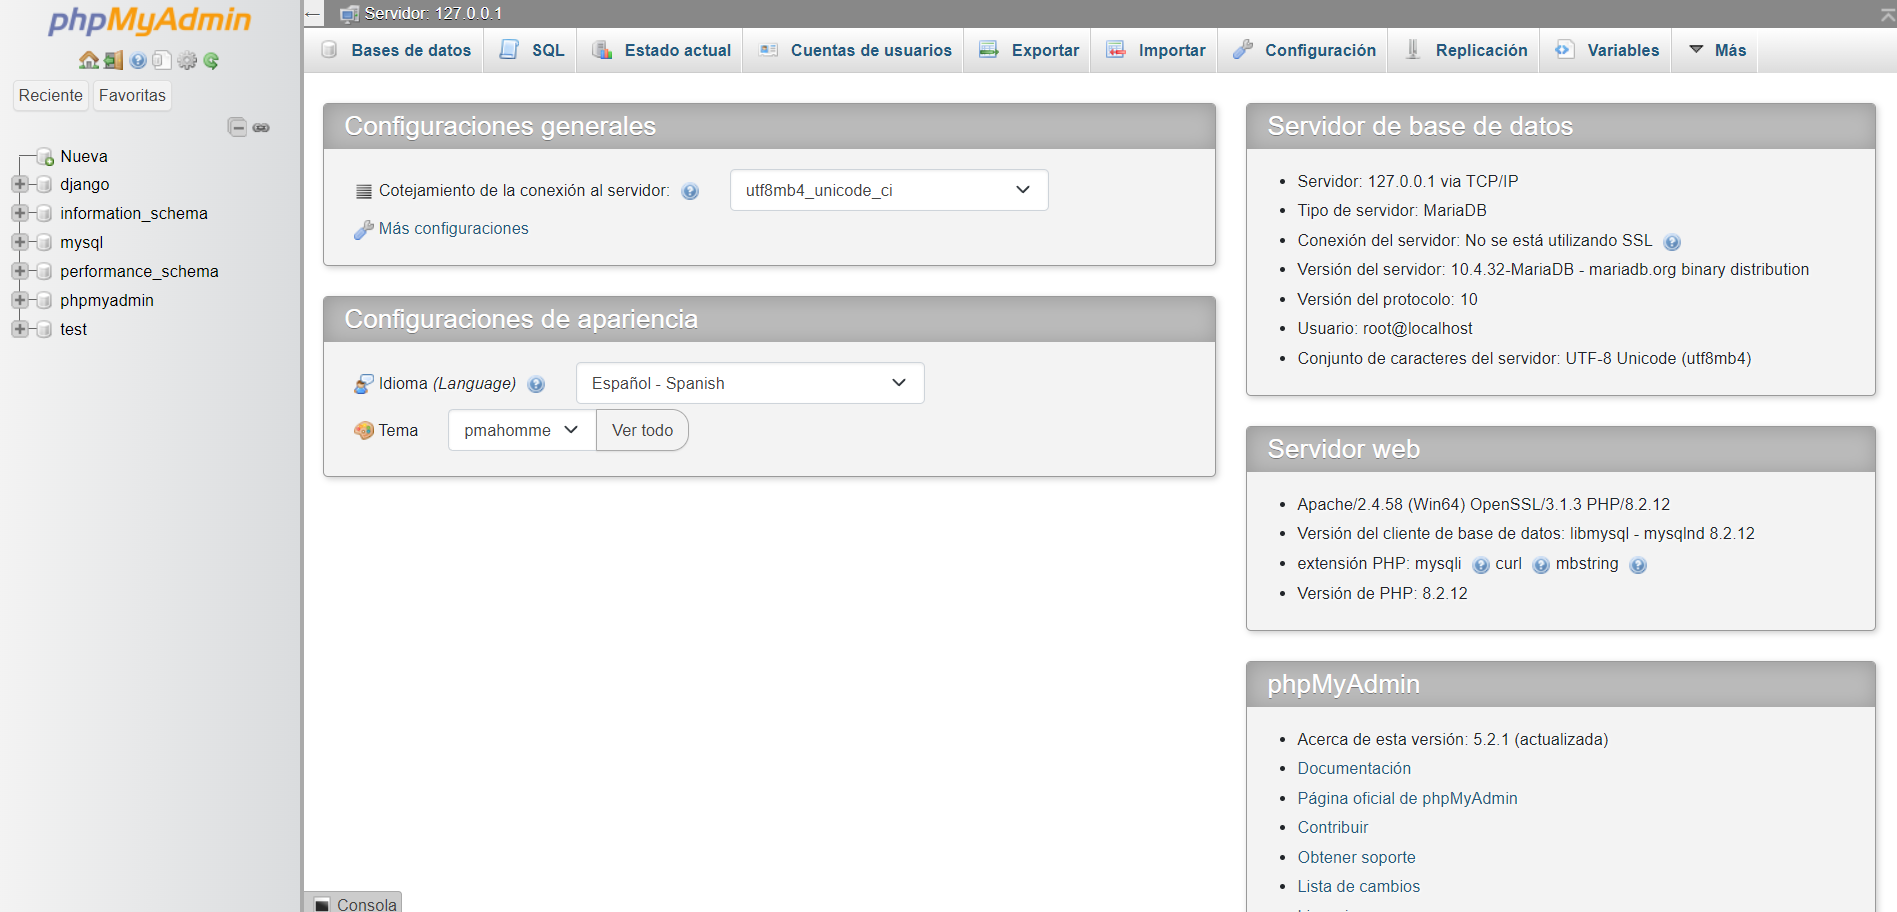
\includegraphics[width=1\textwidth, keepaspectratio]{img/xampp2.png}
      \caption{mySQL - Xampp}
    \end{figure}

%%%%%%%%%%%%%%%%%%%%

  \section{Desarrollo del trabajo}
  
%%%%%%%%%%%%

  \subsection{Relación de uno a muchos: }
  
%%%%%%

  \subsubsection{Vídeo 1: one-to-many-relationships (Proyecto 'model examples')}
    \begin{itemize}
      \item \textbf{Modelos -- Descripcion: }Se define dos modelos en Django que son Language y Framework. 
        El modelo Language tiene un solo campo name que es un CharField con un máximo de 10 caracteres. 
        La representación en forma de cadena del objeto Language devuelve el valor del campo name. El modelo 
        Framework también tiene un campo name que es un CharField con un máximo de 10 caracteres y un campo 
        language que es una clave foránea (ForeignKey) referenciando el modelo Language. La opción on delete=models.CASCADE 
        significa que cuando un objeto Language es eliminado, también se eliminarán todos los objetos Framework asociados a 
        ese lenguaje. La representación en forma de cadena del objeto Framework devuelve el valor del campo name.
        \begin{lstlisting}[language=Python]
          class Language(models.Model):
              name = models.CharField(max_length=10)
              
              def __str__(self):
                  return self.name
              
          class Framework(models.Model):
              name = models.CharField(max_length=10)
              language = models.ForeignKey(Language, on_delete=models.CASCADE)
              
              def __str__(self):
                  return self.name
        \end{lstlisting}
      \item \textbf{Shell -- Descripción: }Lo expresado en el video ilustra cómo manejar relaciones de uno a muchos en Django creando y 
        vinculando objetos de dos modelos distintos: Language y Framework. Inicialmente, se crea una instancia de Language 
        llamada 'Python' y se guarda en la base de datos. Luego, se crean varias instancias de Framework (Django, Flask y Bottle) 
        y se asocian con la instancia de 'Python'. Cada Framework se guarda en la base de datos después de establecer la relación. 
        Más tarde, se crea otra instancia de Language llamada 'Java' y se guarda. Finalmente, se crea una instancia de Framework 
        llamada 'Spring', se asocia con 'Java' y se guarda en la base de datos. Este proceso muestra cómo establecer y guardar 
        relaciones de uno a muchos en Django, donde varios frameworks están asociados con un solo lenguaje.
        \newline
        \begin{lstlisting}
          >>>from example.models import Language, Framework
          >>>python = Language(name='Python')
          >>>python.save()
          >>>django = Framework(name='Django')
          >>>flask = Framework(name='Flask')
          >>>python
          <Language: Language object (1)>
          >>>django.language = python
          >>>flask.language = python
          >>>bottle = Framework(name='Bottle', language=python)
          >>>django.save()
          >>>flask.save()
          >>>bottle.save()
          >>>java = Language(name='Java')
          >>>java.save()
          >>>spring = Framework(name='Spring', language=java)
          >>>spring.save()
        \end{lstlisting}
    \end{itemize}
  
%%%%%%

  \subsubsection{Vídeo 2: Query-one-to-many}
    \begin{itemize}
      \item \textbf{Shell -- Descripción: }Estas consultas de Django empleadas en el video muestran cómo interactuar 
        con modelos relacionados mediante claves foráneas y filtros. Comienza importando los modelos Language y Framework, 
        seguido por una consulta para obtener todos los objetos del modelo Framework. Luego, se aplican filtros para 
        encontrar frameworks según el nombre del lenguaje asociado, devolviendo aquellos relacionados con 'Python' y 'Java'. 
        También se emplean filtros como startswith para buscar lenguajes que empiecen con una determinada cadena. Finalmente, 
        se ejecutan consultas inversas utilizando la clave foránea para encontrar los lenguajes asociados con frameworks 
        específicos, como 'Spring' y 'Bottle'.
        \begin{lstlisting}
          >>> from example.models import Language, Framework
          >>> Framework.objects.all()
          <QuerySet [<Framework: Django>, <Framework: Flask>, <Framework: Bottle>, <Framework: Spring>]>
          >>> Framework.objects.filter(language__name='Python')
          <QuerySet [<Framework: Django>, <Framework: Flask>, <Framework: Bottle>]>
          >>> Framework.objects.filter(language__name='Java')
          <QuerySet [<Framework: Spring>]>
          >>> Framework.objects.filter(language__name__startswith='Py')
          <QuerySet [<Framework: Django>, <Framework: Flask>, <Framework: Bottle>]>
          >>> Framework.objects.filter(language__name__startswith='Pa')
          <QuerySet []>
          >>> Language.objects.filter(framework__name='Spring')
          <QuerySet [<Language: Java>]>
          >>> Language.objects.filter(framework__name='Bottle')
          <QuerySet [<Language: Python>]>
        \end{lstlisting}
    \end{itemize}
  
%%%%%%%%%%%%

  \subsection{Relación muchos a muchos: }
   
%%%%%%

  \subsubsection{Vídeo 3: many-to-many-relationships (Proyecto 'model examples')}
    \begin{itemize}
      \item \textbf{Modelos -- Descripcion: }Estos modelos implementado en el video representan una relación de muchos a muchos 
        entre películas y personajes. El modelo Movie tiene un campo para el nombre de la película y una función str 
        para devolver su nombre como representación legible. Por otro lado, el modelo Character representa personajes con un nombre 
        y una relación de muchos a muchos con películas a través de un campo movies, utilizando el campo ManyToManyField para 
        establecer esta relación. La función str del modelo Character devuelve el nombre del personaje.
        \begin{lstlisting}[language=Python]
          class Movie(models.Model):
              name = models.CharField(max_length=10)
              
              def __str__(self):
                  return self.name
                  
          class Character(models.Model):
              name = models.CharField(max_length=10)
              movies = models.ManyToManyField(Movie)
              
              def __str__(self):
                  return self.name
        \end{lstlisting}
      \item \textbf{Shell -- Descripción: }A continuación se utiliza los modelos Movie y Character de Django 
        para representar relaciones de muchos a muchos entre películas y personajes. Comienza creando una película 
        llamada "Avengers" y un personaje llamado "Captain America", y luego asigna la película "Avengers" al personaje 
        "Captain America". Luego, se crean más películas y personajes, y se establecen relaciones entre ellos mediante 
        el uso de métodos como add() y create() en los campos de relación ManyToManyField. En resumen, este código 
        ilustra cómo trabajar con relaciones de muchos a muchos en un modelo de base de datos utilizando Django.
        \newline
        \begin{lstlisting}
          >>>from example.models import Movie, Character
          >>>avengers = Movie(name='Avengers')
          >>>avengers.save()
          >>>captain_america = Character(name='Captain America')
          >>>captain_america.save()
          >>>captain_america.movies.add(avengers)
          >>>civil_war = Movie(name='Civil War')
          >>>thor = Movie(name='Thor: Dark World')
          >>>thor_character = Character(name='Thor')
          >>>civil_war.save()
          >>>thor.save()
          >>>thor_caracter.save()
          >>>captain_america.movies.add(civil_war)
          >>>thor_character.movies.add(avengers)
          >>>thor_character.movies.add(thor)
          >>captain_america.movies.create(name='Winter Soldier')
          <Movie: Winter Soldier>
        \end{lstlisting}
    \end{itemize}
  
%%%%%%

  \subsubsection{Vídeo 4: many-to-many-Query}
    \begin{itemize}
      \item \textbf{Shell -- Descripción: }En este fragmento se ilustra consultas utilizando relaciones de muchos a muchos 
        entre los modelos Movie (Película) y Character (Personaje). Primero se importan los modelos relevantes del módulo example.models. 
        Luego, se ejecutan varias consultas para buscar información específica en la base de datos. Por ejemplo, se realiza una consulta 
        para encontrar personajes asociados a la película "Civil War" y otra para encontrar películas que incluyan un personaje con el nombre 
        "Captain Am". Estas consultas demuestran cómo utilizar relaciones de muchos a muchos para obtener datos interrelacionados de manera 
        eficiente en Django.
        \begin{lstlisting}
          >>> from example.models import Movie, Character
          >>> Character.objects.filter(movies__name='Civil War')
          <QuerySet [<Character: Captain Am>]>
          >>> Movie.objects.filter(character__name='Captain Am')
          <QuerySet [<Movie: Avengers>, <Movie: Civil War>, <Movie: Winter Sol>]>
          >>> captain_america = Character.objects.get(name='Captain Am')
          >>> captain_america
          <Character: Captain Am>
          >>> captain_america.movies.all()
          <QuerySet [<Movie: Avengers>, <Movie: Civil War>, <Movie: Winter Sol>]>
          >>> avengers = Movie.objects.get(name='Avengers')
          >>> avengers
          <Movie: Avengers>
          >>> avengers.character_set.all()
          <QuerySet [<Character: Captain Am>, <Character: Thor>]>
        \end{lstlisting}
    \end{itemize}
  
%%%%%%%%%%%%

  \subsection{Configuración Base de Datos (Proyecto 'model examples') }
  \textit{Esta configuracion se hace en settings.py, se hizo al iniciar toda la actividad ya que para los primero video se uso mySQL de xampp}
  
%%%%%%

  \subsubsection{Vídeo 5: Database-settings}
    \begin{itemize}
      \item \textbf{Shell -- Descripción: }Este fragmento de configuración se refiere a la configuración de la base de datos en un proyecto Django. 
        Especifica que se está utilizando el motor MySQL para la base de datos por defecto, con el nombre de la base de datos "django", 
        el usuario "Victor", la contraseña "maldonado100204.", el host "localhost" y el puerto "3306".
        \newline
        Para poder usar MySQL en un proyecto Django, es necesario tener instalado el paquete mysqlclient. Este paquete proporciona el 
        adaptador de base de datos necesario para conectar Django con MySQL. Se puedo instalar usando pip: "\texttt{pip install mysqlclient}".
        \begin{figure}[H]
          \centering
          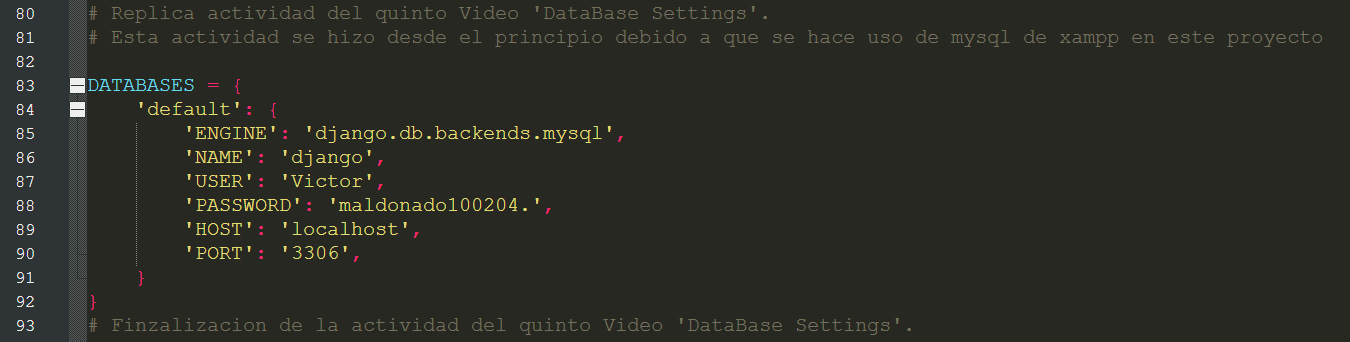
\includegraphics[width=1\textwidth, keepaspectratio]{img/database.png}
          \caption{Configuración Base de Datos - mySQL}
        \end{figure}
    \end{itemize}
  
%%%%%%%%%%%%

  \subsection{Impresión de pdfs (Proyecto 'pdf printing') }
  
%%%%%%

  \subsubsection{Vídeo 6: Render a Django HTML Template to a PDF file Django Utility CFE Render-to-PDF}
    \begin{itemize}
      \item \textbf{VISTAS -- Descripción: }Este siguiente código Django muestra cómo generar un archivo PDF a partir de una plantilla HTML. 
      Primero, se importan las bibliotecas necesarias, se establece la configuración regional para formatear la moneda y se define una clase 
      llamada GeneratePDF que hereda de View.
      \newline
      En el método get, se carga la plantilla HTML utilizando get template y se crea un contexto con datos de ejemplo, como el nombre del 
      cliente, el número de factura, el monto y la fecha. Luego, se renderiza la plantilla con el contexto para obtener el HTML y se utiliza 
      la función 'render to pdf' para convertirlo en un archivo PDF.
      \newline
      Si se genera correctamente el PDF, se crea una respuesta HTTP con el PDF adjunto para descargarlo o visualizarlo en línea, 
      según el parámetro download en la URL. Si no se puede generar el PDF, se devuelve un mensaje de error.
        \begin{lstlisting}[language=Python]
          from django.views.generic import View
          from django.template.loader import get_template
          from .renderers import render_to_pdf
          import locale
          locale.setlocale(locale.LC_ALL, "")

          class GeneratePDF(View):
              def get(self, request, *args, **kwargs):
                  template = get_template('pdf/invoice.html')
                  invoice_number = "007cae"
                  context = {
                      "customer_name": "Ethan Hunt",
                      "invoice_number": f"{invoice_number}",
                      "amount": locale.currency(100_000, grouping=True),
                      "date": "2021-07-04",
                      "pdf_title": f"Invoice #{invoice_number}",
                  }
                  html = template.render(context)
                  pdf = render_to_pdf('pdf/invoice.html', context)
                  if pdf:
                      response = HttpResponse(pdf, content_type='application/pdf')
                      filename = "Invoice_%s.pdf" %("12341231")
                      content = "inline; filename='%s'" %(filename)
                      download = request.GET.get("download")
                      if download:
                          content = "attachment; filename='%s'" %(filename)
                      response['Content-Disposition'] = content
                      return response
                  return HttpResponse('Not Found')
        \end{lstlisting}
      \item \textbf{RENDERERS -- Descripción: }\textit{(Se creo el archivo renderers.py en el proyecto)} Este codigo sirve para 
        convertir una plantilla HTML en un archivo PDF utilizando la librería xhtml2pdf. Se importan módulos como BytesIO para 
        manejar datos binarios, HttpResponse para enviar la respuesta con el PDF, 'get template' para cargar la plantilla HTML, 
        y pisa para la conversión.
        \newline
        La función 'render to pdf' recibe la ruta de la plantilla y un diccionario de contexto opcional. Después de cargar y 
        renderizar la plantilla con el contexto, se utiliza pisa para crear el PDF. Si hay algún problema durante este proceso, 
        se devuelve una respuesta HTTP con el mensaje "Invalid PDF" y un código de estado 400.
        \begin{lstlisting}[language=Python]
          # Video 6 'Render a Django HTML Template to a PDF file Django Utility CFE Render to PDF'
          from io import BytesIO
          from django.http import HttpResponse
          from django.template.loader import get_template

          from xhtml2pdf import pisa

          def render_to_pdf(template_src, context_dict={}):
              template = get_template(template_src)
              html  = template.render(context_dict)
              result = BytesIO()
              pdf = pisa.pisaDocument(BytesIO(html.encode("ISO-8859-1")), result)
              if pdf.err:
                  return HttpResponse("Invalid PDF", status_code=400, content_type='text/plain')
              return HttpResponse(result.getvalue(), content_type='application/pdf')
        \end{lstlisting}
      \item \textbf{URLS -- Descripción: }El siguiente código define las URL de un proyecto Django. Al acceder a la URL /pdf/, 
        se activa la vista GeneratePDF que está definida en el archivo de vistas (views.py). Esta vista se encarga de generar 
        un archivo PDF a partir de una plantilla HTML y enviarlo como respuesta.
        \begin{lstlisting}[language=Python]
          from django.contrib import admin
          from django.urls import path
          from .views import GeneratePDF

          urlpatterns = [
              path('admin/', admin.site.urls),
              path('pdf/', GeneratePDF.as_view()),
          ]
        \end{lstlisting}
      \item \textbf{Plantilla invoice.html -- Descripción: }Este fragmento de código representa una plantilla HTML para generar 
        facturas en un proyecto Django. Incluye estilos CSS para dar formato al contenido, como el tamaño y el color de la fuente, 
        así como la alineación del texto. Utiliza variables del contexto, como 'invoice number', 'customer name', amount, y date, 
        para personalizar la información de cada factura generada en PDF.
        \begin{lstlisting}[language=HTML]
          <!-- Video 6 'Render a Django HTML Template to a PDF file Django Utility CFE Render to PDF' -->
          <!DOCTYPE HTML PUBLIC "-//W3C//DTD HTML 4.01 Transitional//EN" "http://www.w3.org/TR/html4/loose.dtd">
          <html>
            <head>
              <title>New Title Here</title>
              <style type="text/css">
                body {
                  font-weight: 200;
                  font-size: 14px;
                }
                .header {
                  font-size: 20px;
                  font-weight: 100;
                  text-align: center;
                  color: #007cae;
                }
                .title {
                  font-size: 22px;
                  font-weight: 100;
                  padding: 10px 20px 0px 20px;
                }
                .title span {
                  color: #007cae;
                }
                .details {
                  padding: 10px 20px 0px 20px;
                  text-align: left !important;
                }
                .hrItem {
                  border: none;
                  height: 1px;
                  color: #333;
                  background-color: #fff;
                }
              </style>
            </head>
            <body>
              <div class='wrapper'>
                <div class='header'>
                  <p class='title'>Invoice #{{ invoice_number}}</p>
                </div>
                <div class='details'>
                  Bill to: {{ customer_name }}<br/>
                  Amount: {{ amount }} <br/>
                  Date: {{ date }}
                  <hr class='hrItem' />
                </div>
              </div>
            </body>
          </html>
        \end{lstlisting}
      \newpage
      \item \textbf{Ejecución: }
        \begin{figure}[H]
          \centering
          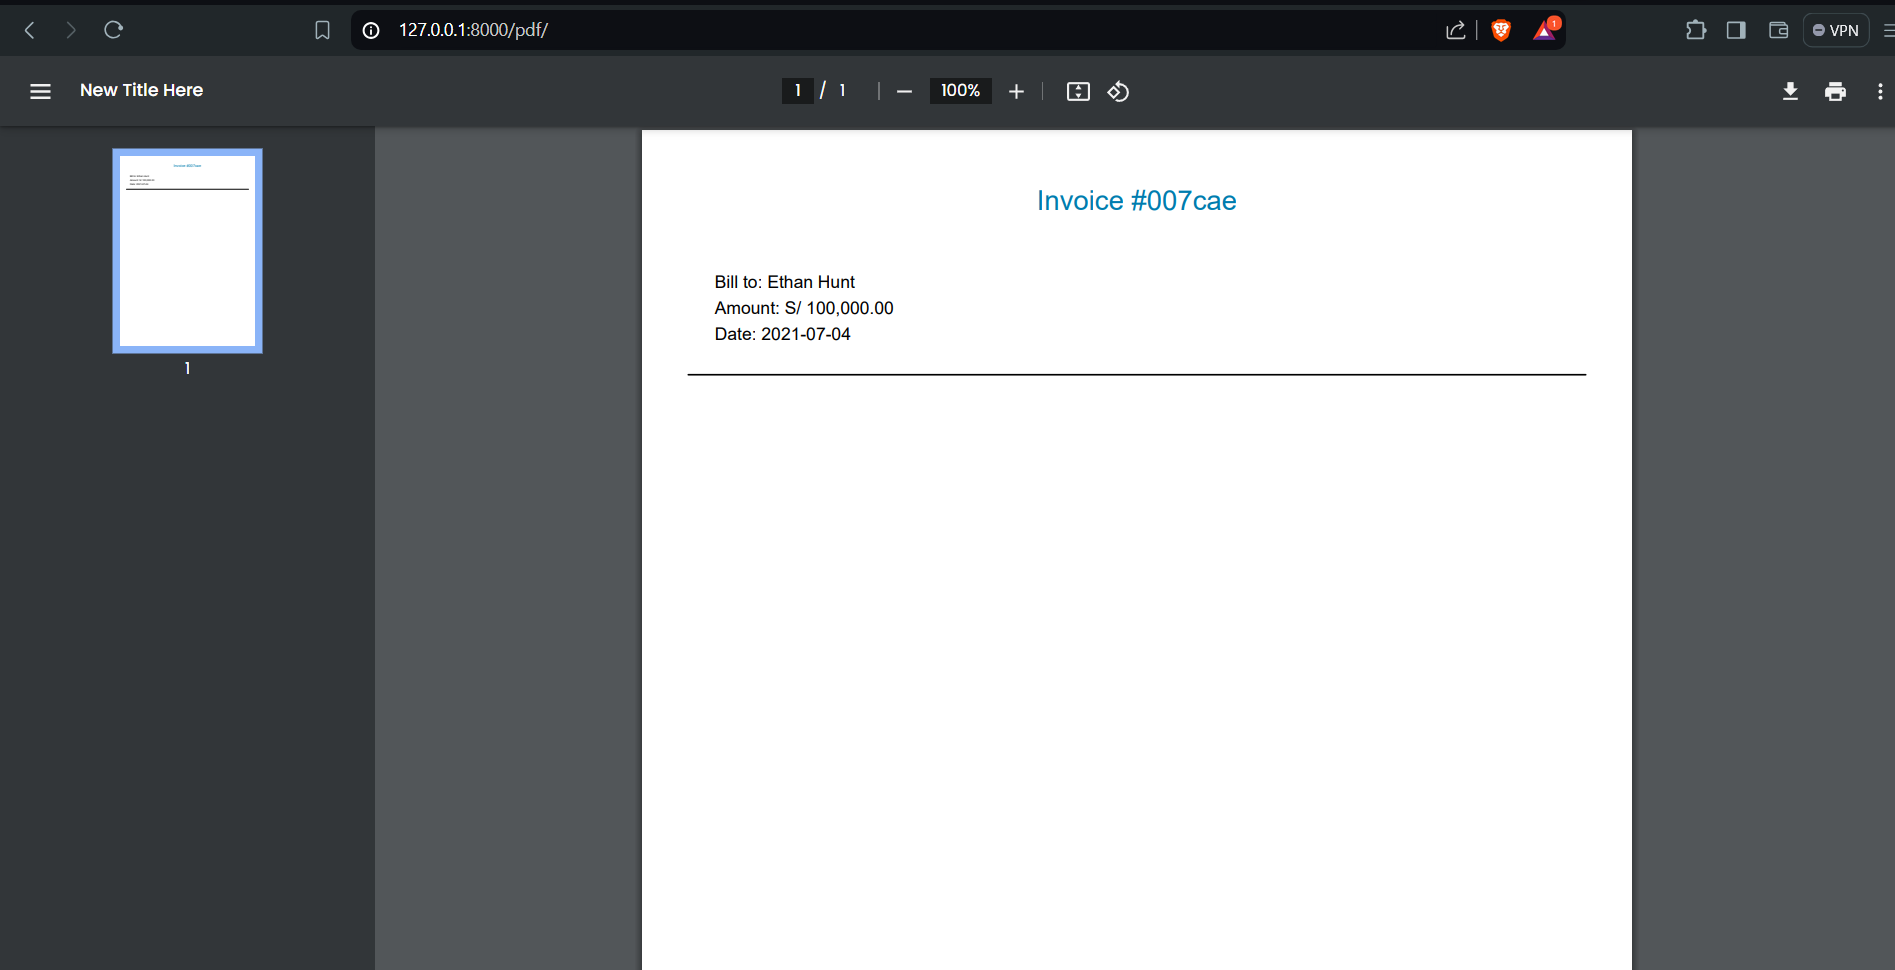
\includegraphics[width=1\textwidth, keepaspectratio]{img/ejecucion1.png}
          \caption{Ejecución}
        \end{figure}
        \begin{figure}[H]
          \centering
          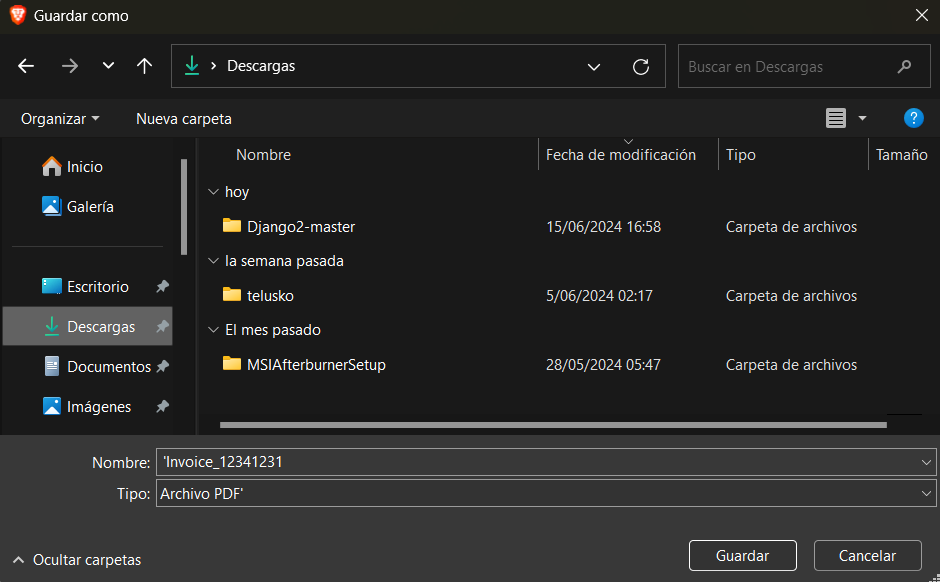
\includegraphics[width=1\textwidth, keepaspectratio]{img/ejecucion2.png}
          \caption{Ejecución}
        \end{figure}
        \begin{figure}[H]
          \centering
          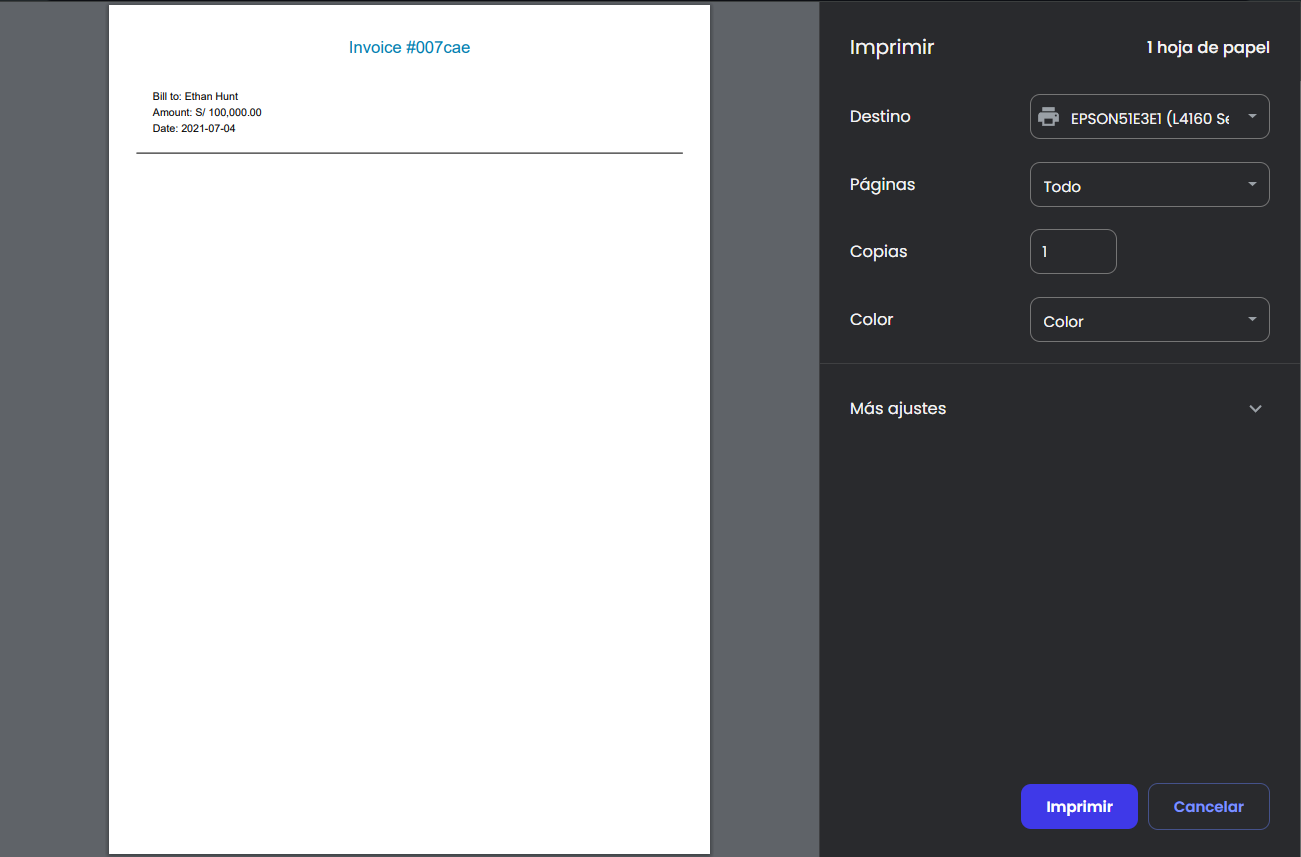
\includegraphics[width=1\textwidth, keepaspectratio]{img/ejecucion3.png}
          \caption{Ejecución}
        \end{figure}
    \end{itemize}
  
%%%%%%%%%%%%

  \subsection{Envio de emails (Proyecto 'email project')}
  
%%%%%%

  \subsubsection{Vídeo 7: Sending Emails in Django}
    \begin{itemize}
        \item \textbf{Configuración de email en setting.py: } 
          \begin{figure}[H]
            \centering
            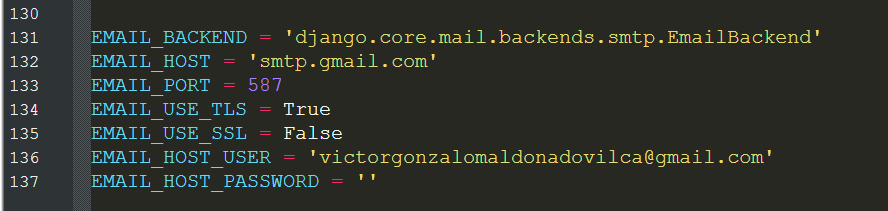
\includegraphics[width=1\textwidth, keepaspectratio]{img/emailconf.png}
            \caption{Configuración}
          \end{figure}
        \item \textbf{VISTAS -- Descripción: }En este fragmento de código se muestra cómo enviar un correo electrónico desde una vista. 
          Utiliza la función 'send mail' para enviar un saludo simple ("Hola Mundo!!") desde la dirección de correo electrónico 
          'victorgonzalomaldonadovilca@gmail.com' a 'vmaldonadov@unsa.edu.pe'. Luego, renderiza una plantilla HTML para la página de 
          índice ('index.html').
          \begin{lstlisting}[language=Python]
            from django.shortcuts import render
            from django.core.mail import send_mail

            # Create your views here.

            def index(request):
                send_mail(
                    'Saludo desde Django',
                    'Hola Mundo!!',
                    'victorgonzalomaldonadovilca@gmail.com',
                    ['vmaldonadov@unsa.edu.pe'],
                )
                return render(request, "email/index.html")
          \end{lstlisting}
        \item \textbf{URLS (Project) -- Descripción: }El siguiente código configura las rutas del proyecto Django. Conecta la URL 'admin/' 
          al panel de administración de Django y la URL principal ('') a las rutas definidas en 'email app.urls', permitiendo acceder al panel 
          de administración y a las vistas de la aplicación 'email app' a través de las rutas correspondientes en esos archivos.
          \begin{lstlisting}[language=Python]
            from django.contrib import admin
            from django.urls import path, include

            urlpatterns = [
                path('admin/', admin.site.urls),
                path('', include('email_app.urls')),
            ]
          \end{lstlisting}
        \item \textbf{URLS (APP) -- Descripción: }El código define las rutas de la aplicación Django. Enlaza la URL principal con 
          la vista 'index' de la aplicación actual ('.'). Esto permite acceder a la vista 'index' al ingresar a la URL principal del proyecto.
          \begin{lstlisting}[language=Python]
            # Video 7 'Sending Emails in Django'

            from django.urls import path
            from . import views

            urlpatterns = [
                path('', views.index)
            ]
          \end{lstlisting}
        \item \textbf{Plantilla index.html -- Descripción: }Este código HTML crea una página básica que muestra un encabezado que 
          dice "Send a Email".
          \begin{lstlisting}[language=Python]
            <!DOCTYPE HTML>
            <html>
              <head>
                <meta charset="UTF-8"/>
                <meta name="viewport" content="width=device-width, initial-scale=1.0"/>
              </head>
              <body>
                <h1>Send a Email</h1>
              </body>
            </html>
          \end{lstlisting}
        \item \textbf{Ejecución: }
          \begin{figure}[H]
            \centering
            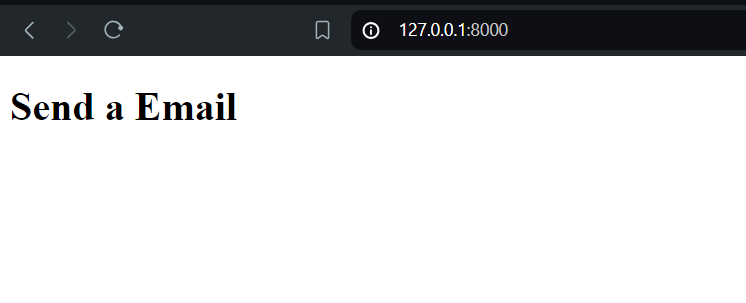
\includegraphics[width=1\textwidth, keepaspectratio]{img/ejecucion4.png}
            \caption{Ejecución}
          \end{figure}
          \begin{figure}[H]
            \centering
            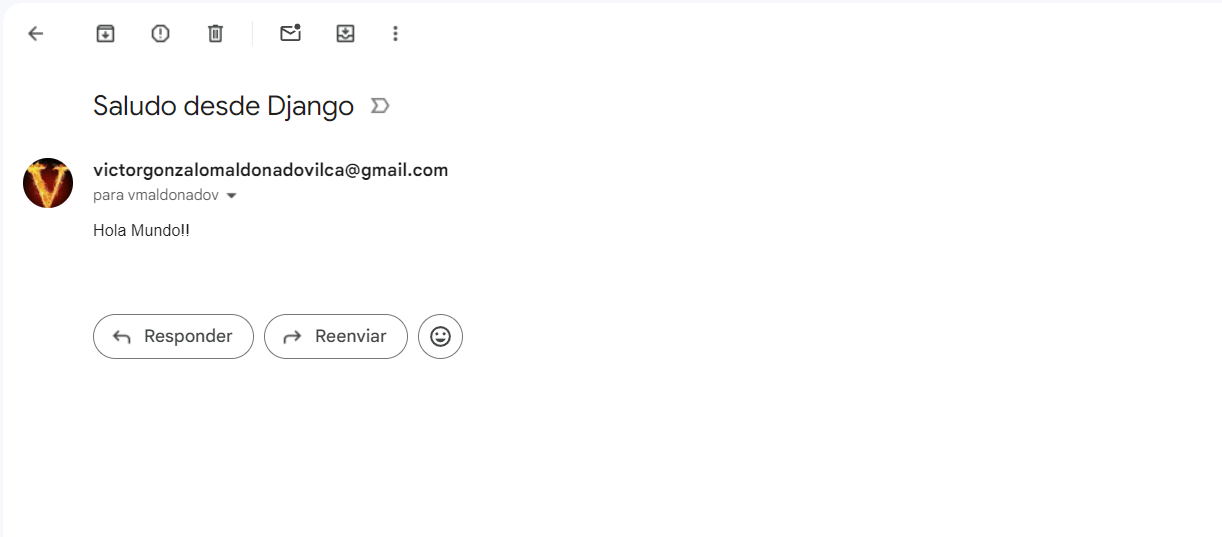
\includegraphics[width=1\textwidth, keepaspectratio]{img/ejecucion5.png}
            \caption{Ejecución - Emisor}
          \end{figure}
          \begin{figure}[H]
            \centering
            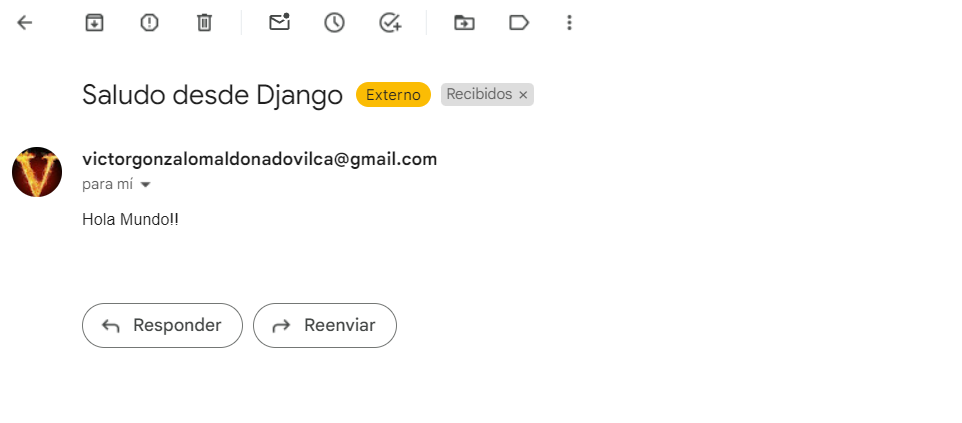
\includegraphics[width=1\textwidth, keepaspectratio]{img/ejecucion6.png}
            \caption{Ejecución - Receptor}
          \end{figure}
      \end{itemize}

%%%%%%%%%%%%%%%%%%%%
	
  \subsection{Uso de GitHub}
  
%%%%%%%%%%%%%%%%%%%%

	\subsubsection{Usuario de GitHub}
    \begin{figure}[H]
      \centering
      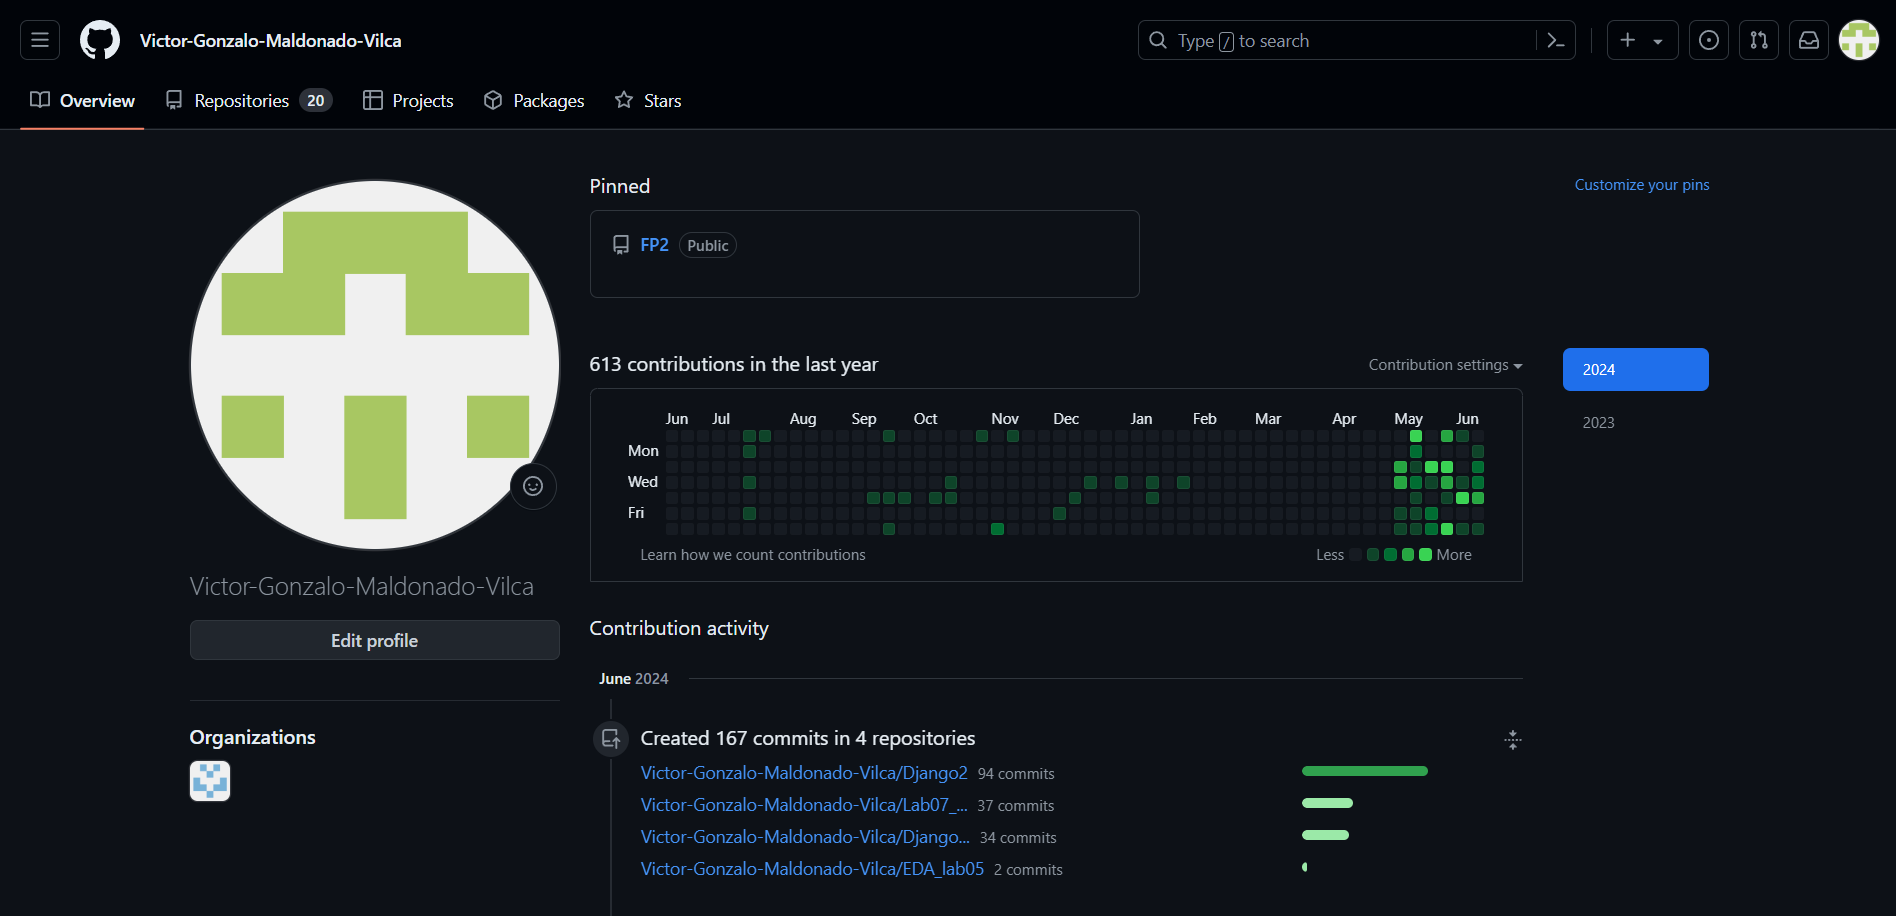
\includegraphics[width=1\textwidth, keepaspectratio]{img/usuario.png}
      \caption{Usuario}
    \end{figure}
  
%%%%%%%%%%%%%%%%%%%%  
  
  \subsubsection{Implementación de Readme.md}
    \begin{figure}[H]
      \centering
      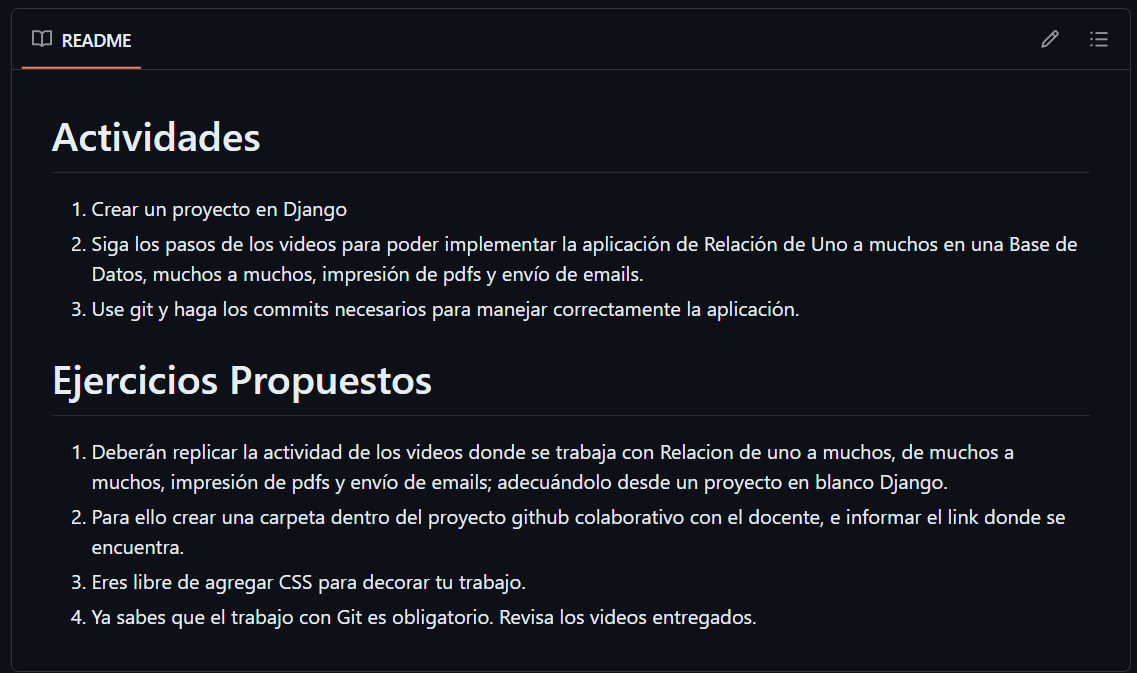
\includegraphics[width=1\textwidth, keepaspectratio]{img/readme.png}
      \caption{README.md}
    \end{figure}
  
%%%%%%%%%%%%%%%%%%%%

	\subsubsection{Registro de cambios en mi código}
    \begin{figure}[H]
      \centering
      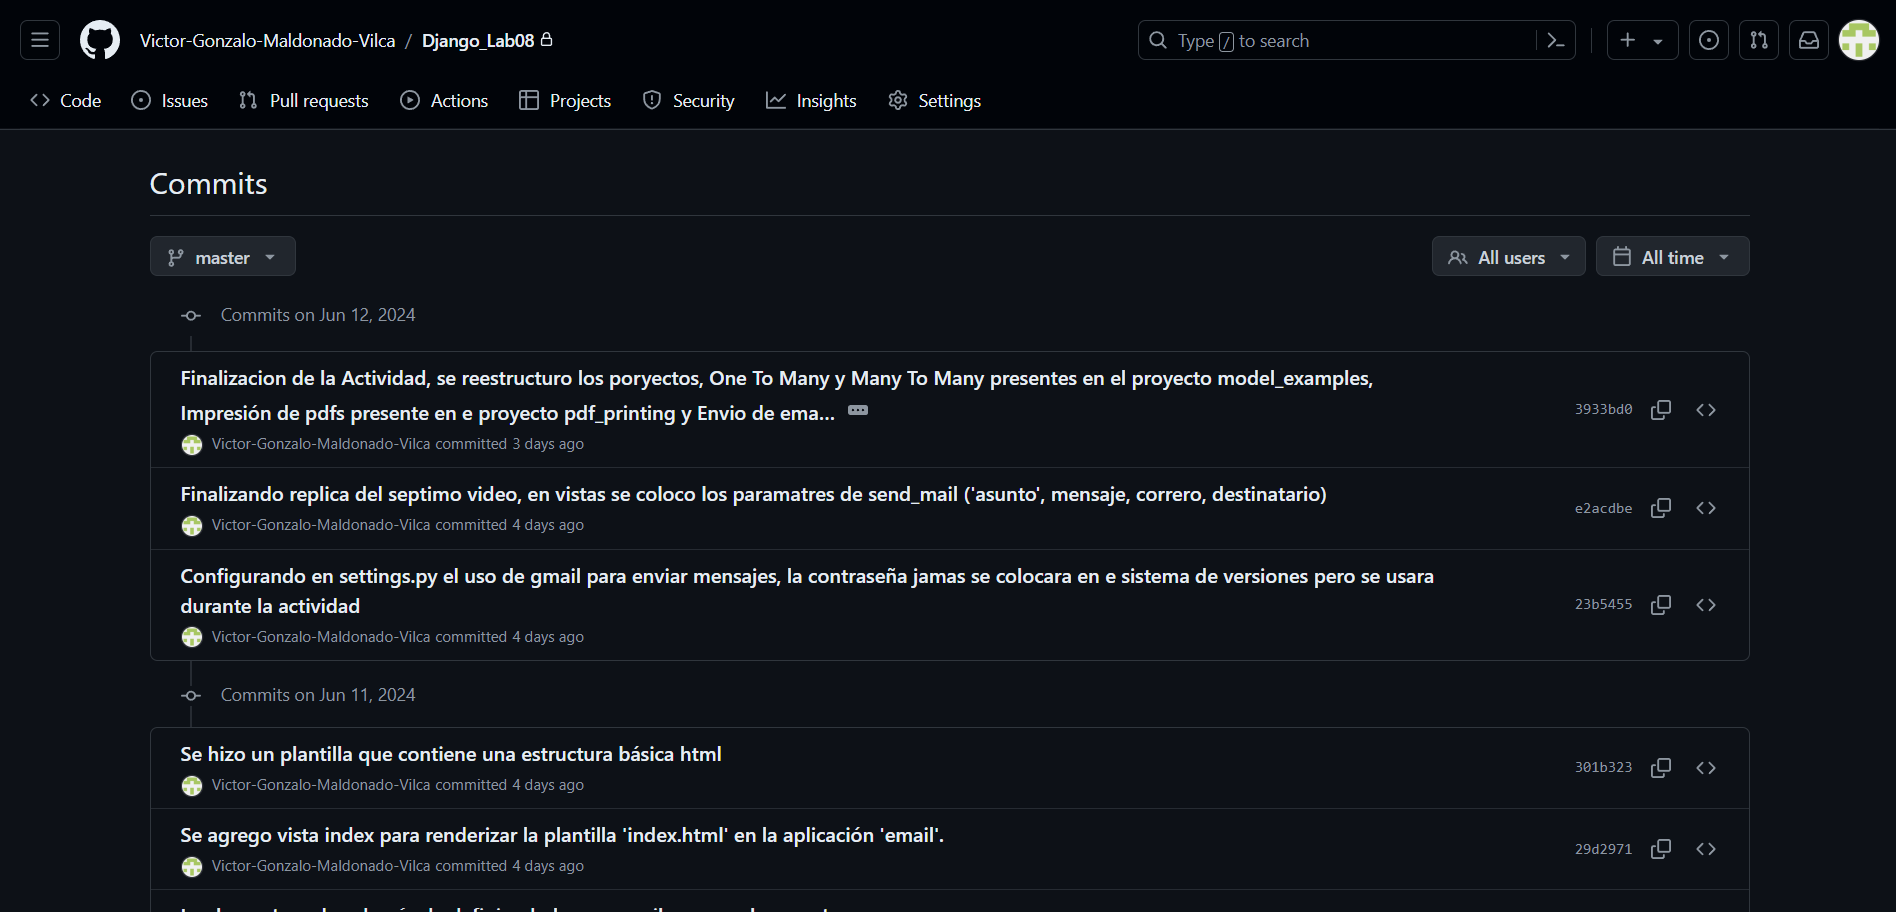
\includegraphics[width=1\textwidth, keepaspectratio]{img/commits.png}
      \caption{Commits}
    \end{figure}
	
%%%%%%%%%%%%%%%%%%%%

	\subsubsection{Repositorio}
    \begin{figure}[H]
      \centering
      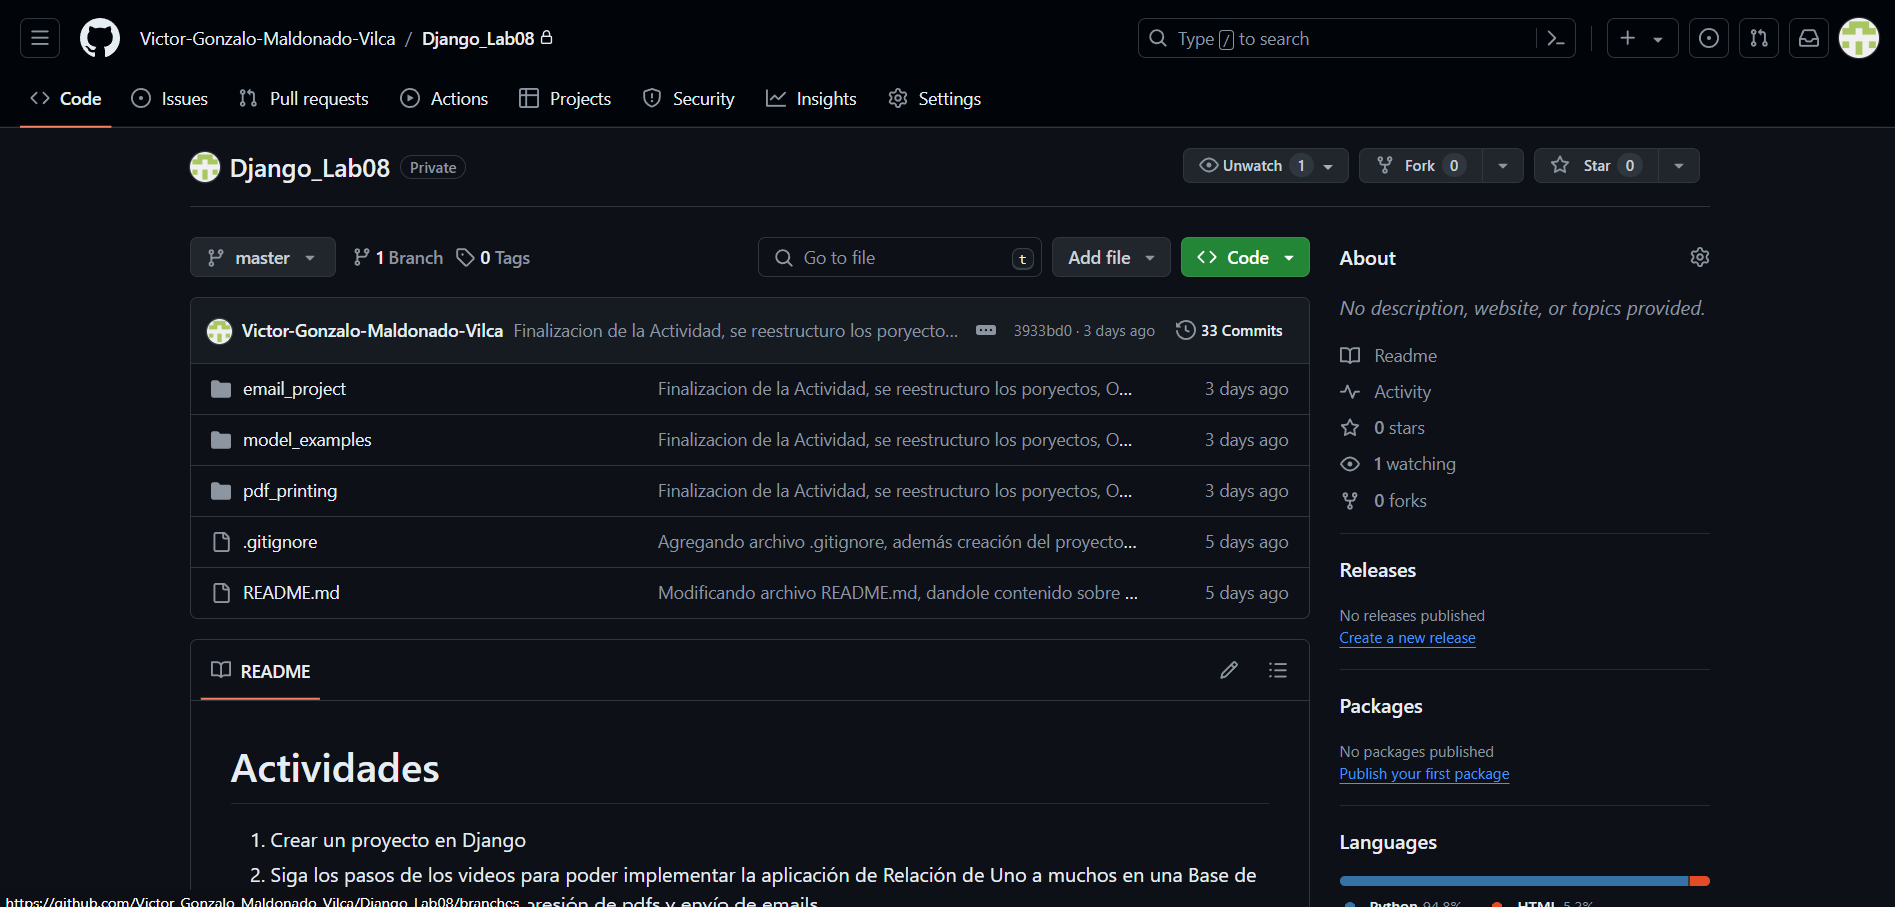
\includegraphics[width=1\textwidth, keepaspectratio]{img/repositorio.png}
      \caption{Repositorio}
    \end{figure}
  
%%%%%%%%%%%%%%%%%%%%

	\subsubsection{Proyecto compartido con el profesor de github}
    \begin{figure}[H]
      \centering
      \includegraphics[width=1\textwidth, keepaspectratio]{img/Compartir.png}
      \caption{Compartir con el Docente}
    \end{figure}
  \newpage
  
%%%%%%%%%%%%%%%%%%%%

  \section{Recomensaciones}
  \begin{itemize}
    \item Utiliza las relaciones de uno a muchos (\texttt{ForeignKey}) y muchos a muchos (\texttt{ManyToManyField}) de manera adecuada según la estructura de tus datos. Esto te permitirá organizar y gestionar la información de forma eficiente.
    \item Al imprimir PDFs, asegúrate de utilizar bibliotecas como xhtml2pdf o ReportLab para generar documentos de alta calidad y compatibles con diferentes dispositivos y navegadores.
    \item Al enviar emails, verifica que la configuración de SMTP en Django esté correctamente establecida y que los correos se envíen de manera segura para evitar problemas de entrega.
  \end{itemize}

%%%%%%%%%%%%%%%%%%%%

  \section{Conclusiones}
  \begin{itemize}
    \item Las relaciones de uno a muchos y muchos a muchos son fundamentales en el diseño de bases de datos relacionales en Django, facilitando la organización y asociación de los datos entre diferentes modelos.
    \item La generación de PDFs y el envío de emails son funcionalidades potentes que amplían las capacidades de una aplicación Django, permitiendo la entrega de información en formatos estáticos y dinámicos.
    \item Es importante considerar aspectos de seguridad y rendimiento al implementar la impresión de PDFs y el envío de emails para garantizar una experiencia óptima para los usuarios finales.
  \end{itemize}

%%%%%%%%%%%%%%%%%%%%
	\newpage
	\subsection{\textcolor{red}{Rúbrica para el contenido del Informe y demostración}}
	\begin{itemize}			
		\item El alumno debe marcar o dejar en blanco en celdas de la columna \textbf{Checklist} si cumplio con el ítem correspondiente.
		\item Si un alumno supera la fecha de entrega,  su calificación será sobre la nota mínima aprobada, siempre y cuando cumpla con todos lo items.
		\item El alumno debe autocalificarse en la columna \textbf{Estudiante} de acuerdo a la siguiente tabla:
	
		\begin{table}[ht]
			\caption{Niveles de desempeño}
			\begin{center}
			\begin{tabular}{ccccc}
    			\hline
    			 & \multicolumn{4}{c}{Nivel}\\
    			\cline{1-5}
    			\textbf{Puntos} & Insatisfactorio 25\%& En Proceso 50\% & Satisfactorio 75\% & Sobresaliente 100\%\\
    			\textbf{2.0}&0.5&1.0&1.5&2.0\\
    			\textbf{4.0}&1.0&2.0&3.0&4.0\\
    		\hline
			\end{tabular}
		\end{center}
	\end{table}	
	

	\end{itemize}

 
	
	\begin{table}[H]
		\caption{Rúbrica para contenido del Informe y demostración}
		\setlength{\tabcolsep}{0.5em} % for the horizontal padding
		{\renewcommand{\arraystretch}{1.5}% for the vertical padding
		%\begin{center}
		\begin{tabular}{|p{2.7cm}|p{7cm}|x{1.3cm}|p{1.2cm}|p{1.5cm}|p{1.1cm}|}
			\hline
    		\multicolumn{2}{|c|}{Contenido y demostración} & Puntos & Checklist & Estudiante & Profesor\\
			\hline
			\textbf{1. GitHub} & Hay enlace URL activo del directorio para el  laboratorio hacia su repositorio GitHub con código fuente terminado y fácil de revisar. &2 &X &2 & \\ 
			\hline
			\textbf{2. Commits} &  Hay capturas de pantalla de los commits más importantes con sus explicaciones detalladas. (El profesor puede preguntar para refrendar calificación). &4 &X &4 & \\ 
			\hline 
			\textbf{3. Código fuente} &  Hay porciones de código fuente importantes con numeración y explicaciones detalladas de sus funciones. &2 &X &2 & \\ 
			\hline 
			\textbf{4. Ejecución} & Se incluyen ejecuciones/pruebas del código fuente  explicadas gradualmente. &2 &X &2 & \\ 
			\hline			
			\textbf{5. Pregunta} & Se responde con completitud a la pregunta formulada en la tarea.  (El profesor puede preguntar para refrendar calificación).  &2 &X &2 & \\ 
			\hline	
			\textbf{6. Fechas} & Las fechas de modificación del código fuente estan dentro de los plazos de fecha de entrega establecidos. &2 &X &2 & \\ 
			\hline 
			\textbf{7. Ortografía} & El documento no muestra errores ortográficos. &2 &X &2 & \\ 
			\hline 
			\textbf{8. Madurez} & El Informe muestra de manera general una evolución de la madurez del código fuente,  explicaciones puntuales pero precisas y un acabado impecable.   (El profesor puede preguntar para refrendar calificación).  &4 &X &4 & \\ 
			\hline
			\multicolumn{2}{|c|}{\textbf{Total}} &20 & &20 & \\ 
			\hline
		\end{tabular}
		%\end{center}
		%\label{tab:multicol}
		}
	\end{table}


%%%%%%%%%%%%%%%%%%%%%%%%%%%%%%%%%%%%%%%%%%%%%%%%%%%%%%%%%%%%%%%%%%%
	
  \newpage
  \section{Referencias}
    \begin{itemize}
      \item \url{https://docs.djangoproject.com/es/3.2/}
      \item \url{https://docs.djangoproject.com/en/5.0/}
      \item \url{https://docs.github.com/es}
      \item \url{https://git-scm.com/doc}
    \end{itemize}

%%%%%%%%%%%%%%%%%%%% 
%\clearpage
%\bibliographystyle{apalike}
%\bibliographystyle{IEEEtranN}
%\bibliography{bibliography}
			
\end{document}
